\documentclass[10pt]{beamer}

\usetheme[progressbar=frametitle]{metropolis}

\usepackage[utf8]{inputenc}
\usepackage[spanish]{babel}
\usepackage{booktabs}
\usepackage{graphicx}
\usepackage{subcaption}
\usepackage{animate}
\metroset{block=fill}

\newcommand\blfootnote[1]{%
  \begingroup
  \renewcommand\thefootnote{}\footnote{#1}%
  \addtocounter{footnote}{-1}%
  \endgroup
}

\title{Aprendizaje profundo para el análisis de comportamientos en
  videovigilancia}
\subtitle{Trabajo de Fin de Máster}
\date{\today}
\author{Francisco Luque Sánchez}
\institute{Universidad de Granada - Máster en Ciencia de Datos
  e Ingeniería de Computadores}

\begin{document}

\maketitle

\begin{frame}{Índice}
  \setbeamertemplate{section in toc}[sections numbered]
  \tableofcontents[hideallsubsections]
\end{frame}

\section{Descripción del problema}

\begin{frame}{Descripción del problema}
  \begin{block}{Detección de comportamientos anómalos en multitudes}
    \begin{itemize}
    \item Estudio de secuencias de vídeo.
    \item Extraídas de cámaras de videovigilancia.
    \item Análisis de comportamientos.
    \item Idenficación de comportamientos extraños.
    \item Problema complejo y de gran variabilidad.
    \end{itemize}
  \end{block}
\end{frame}

\section{Revisión bibliográfica y taxonomía}

\begin{frame}{Revisión de la literatura}
  \begin{block}{Detección de comportamientos anómalos}
    \begin{itemize}
    \item Categorización de las anomalías por tipos (acciones,
      movimientos, apariencia).
    \item Conjuntos de datos públicos.
    \item Modelos basados en aprendizaje profundo.
    \end{itemize}
  \end{block}
\end{frame}

\begin{frame}{Propuesta taxonómica}
  \begin{figure}
    \centering
    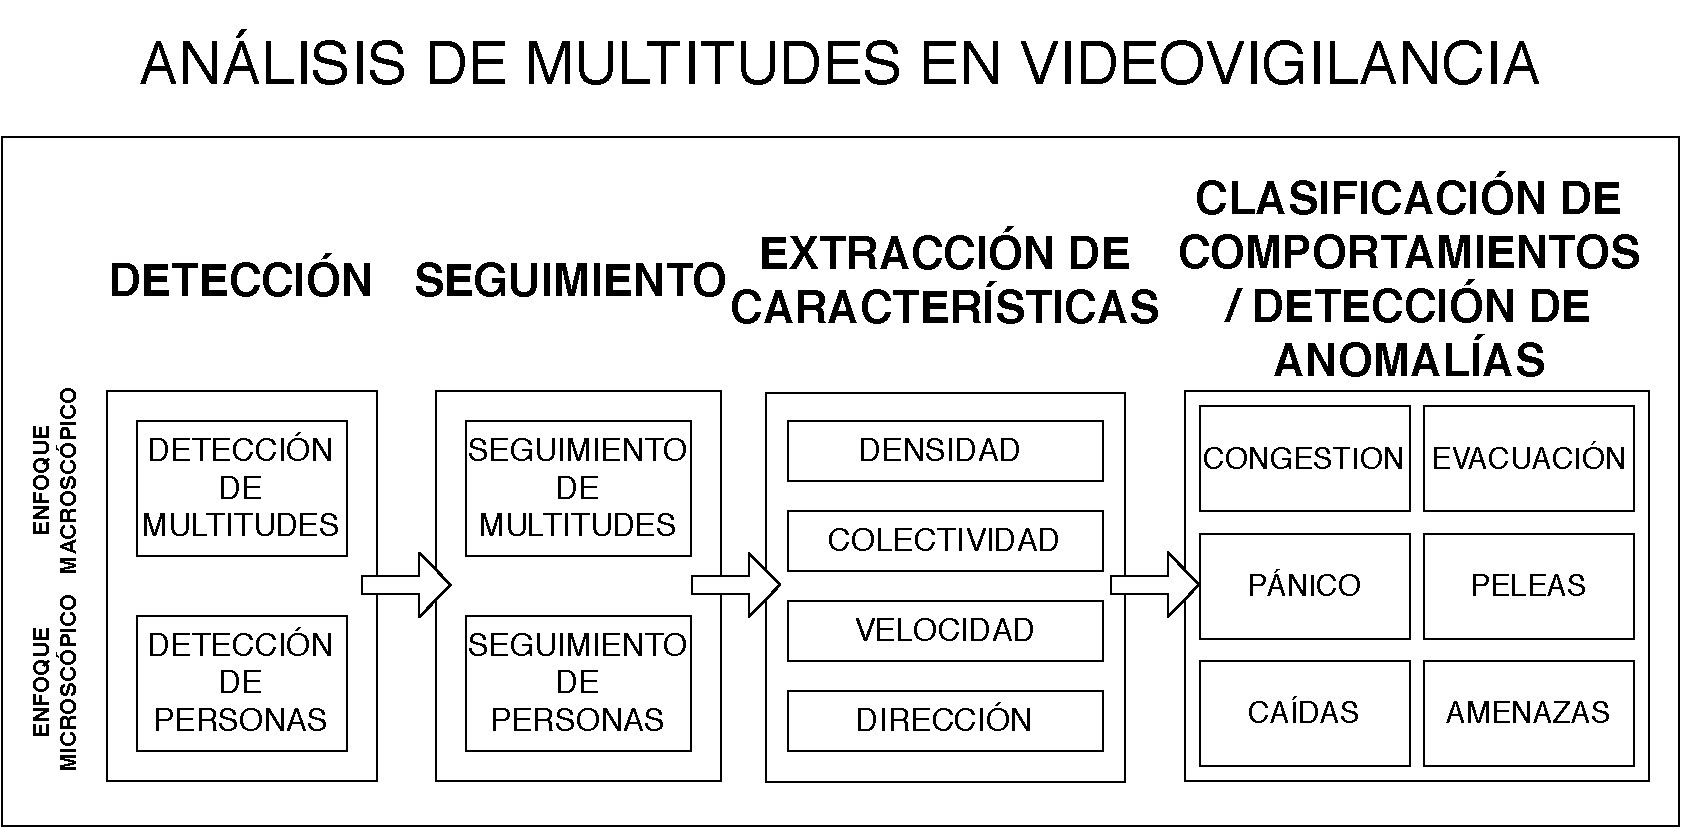
\includegraphics[width=.7\textwidth]{images/taxonomy-steps.pdf}
    \caption{Taxonomía secuencial para el análisis de multitudes}
  \end{figure}

  \blfootnote{\textbf{Luque-Sánchez, F.}, Hupont, I., Tabik, S., \& Herrera,
    F. (2020). Revisiting crowd behaviour analysis through deep
    learning: Taxonomy, anomaly detection, crowd emotions, datasets,
    opportunities and prospects. \textit{Information Fusion}}
\end{frame}

\section{Detección de anomalías en videovigilancia}

\begin{frame}{Hipótesis de partida}
  \begin{block}{Hipótesis}
    Los extractores de características espacio-temporales (CNN+LSTM)
    obtienen características de calidad para detectar comportamientos
    anómalos.
  \end{block}
\end{frame}

\begin{frame}{UCF-Crime Dataset}
  \begin{block}{Características}
    \begin{itemize}
    \item 1900 vídeos
    \item 128 horas en total
    \item 13 clases de comportamientos anómalos
    \item Etiquetado débil
    \end{itemize}
  \end{block}
\end{frame}

\begin{frame}{UCF-Crime Dataset}
  \begin{figure}[hbtp]
    \centering
    \begin{subfigure}{0.35\textwidth}
      \centering
      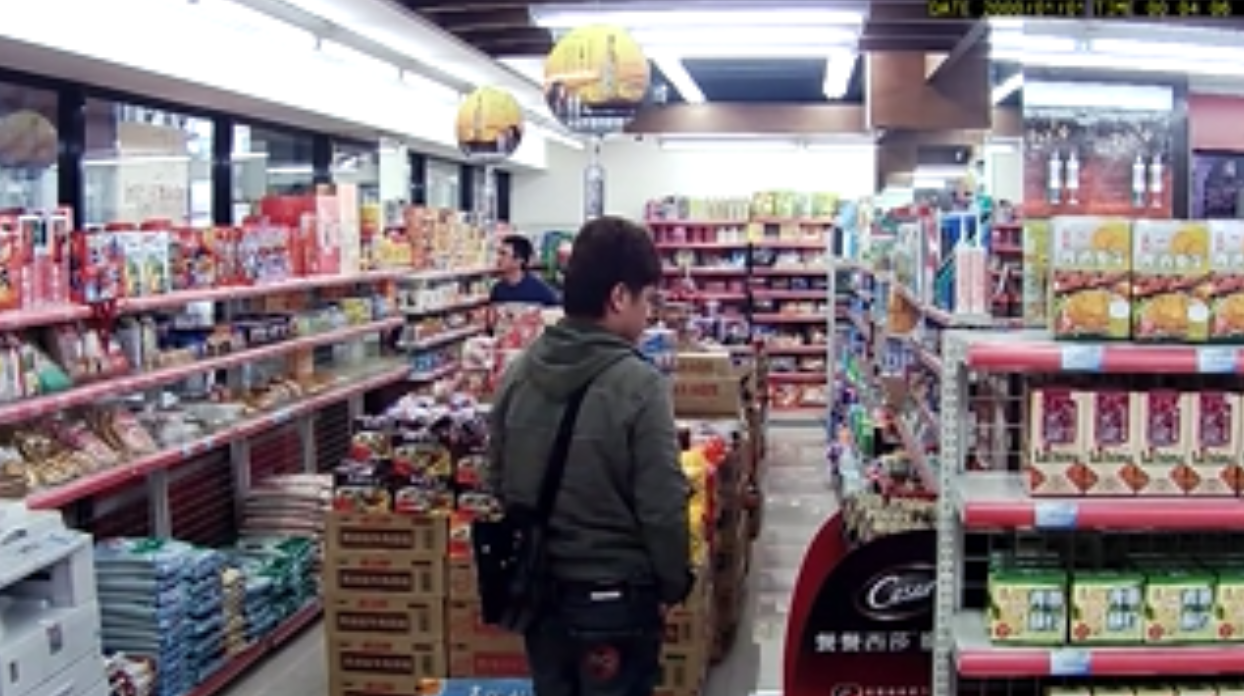
\includegraphics[width=\linewidth]{images/ucf/normal-1}
      \caption{Vídeo normal}
    \end{subfigure}
    \begin{subfigure}{0.35\textwidth}
      \centering
      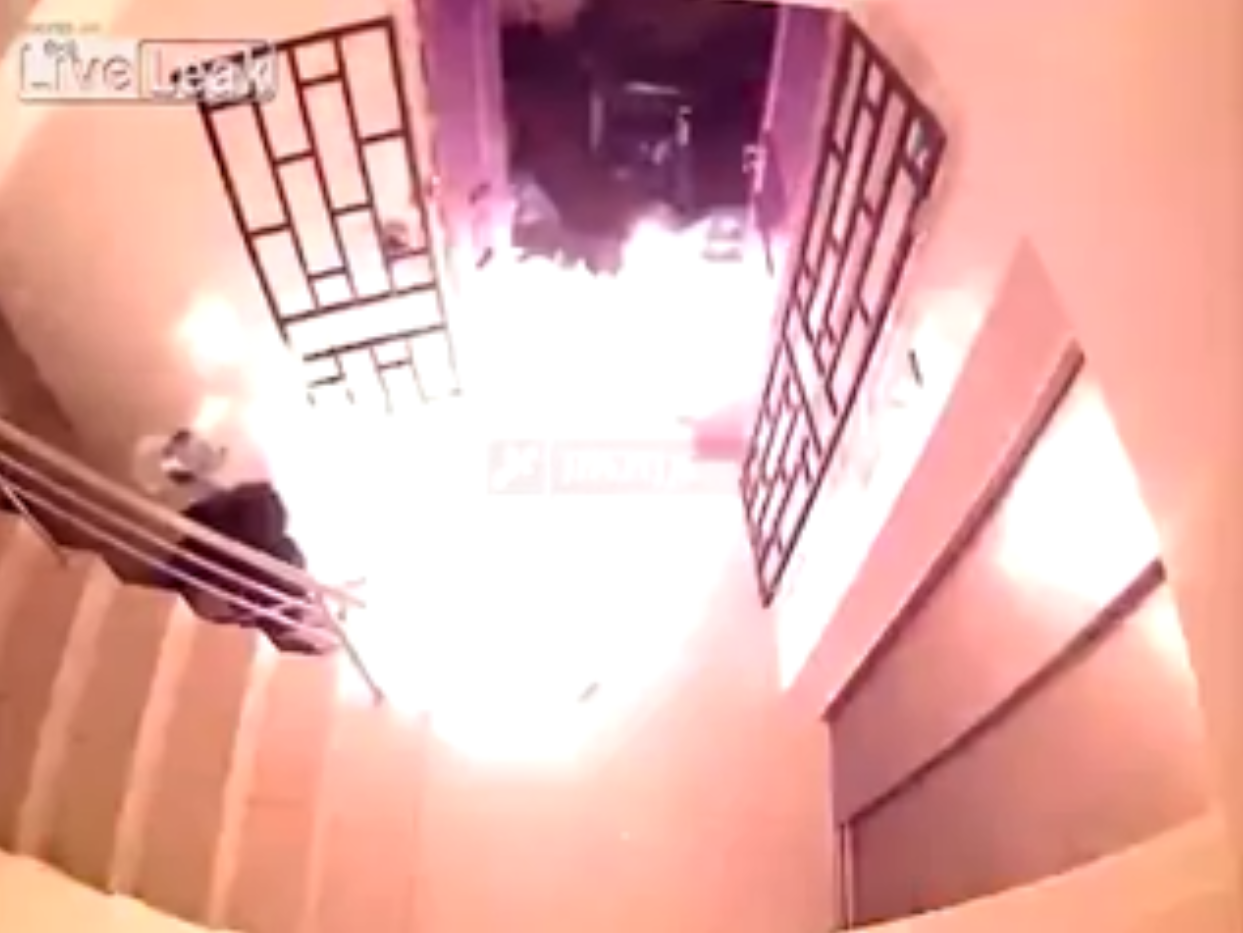
\includegraphics[width=\linewidth]{images/ucf/arson-abnormal}
      \caption{Fuego provocado}
    \end{subfigure}
    \begin{subfigure}{0.35\textwidth}
      \centering
      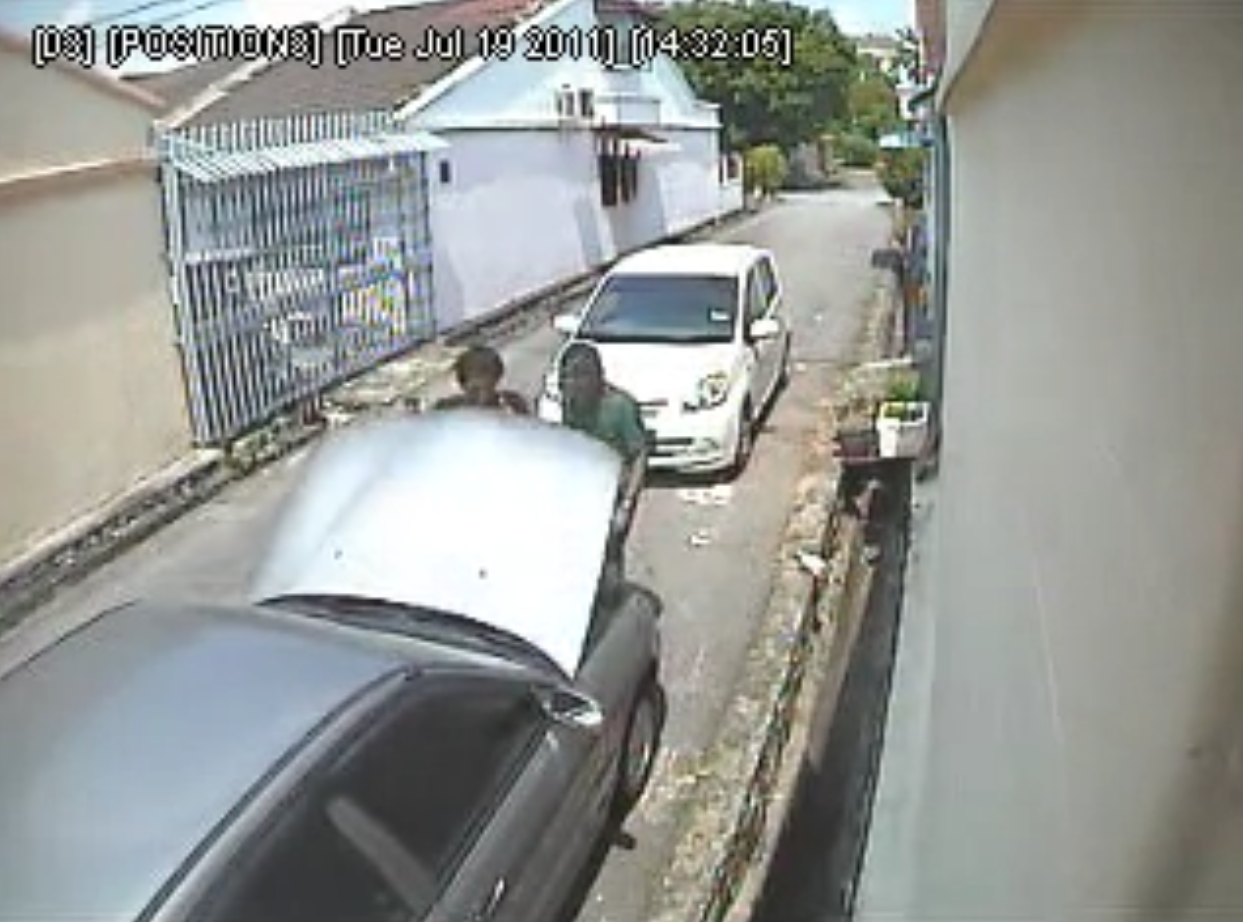
\includegraphics[width=\linewidth]{images/ucf/stealing-abnormal}
      \caption{Robo}
    \end{subfigure}
    \begin{subfigure}{0.35\textwidth}
      \centering
      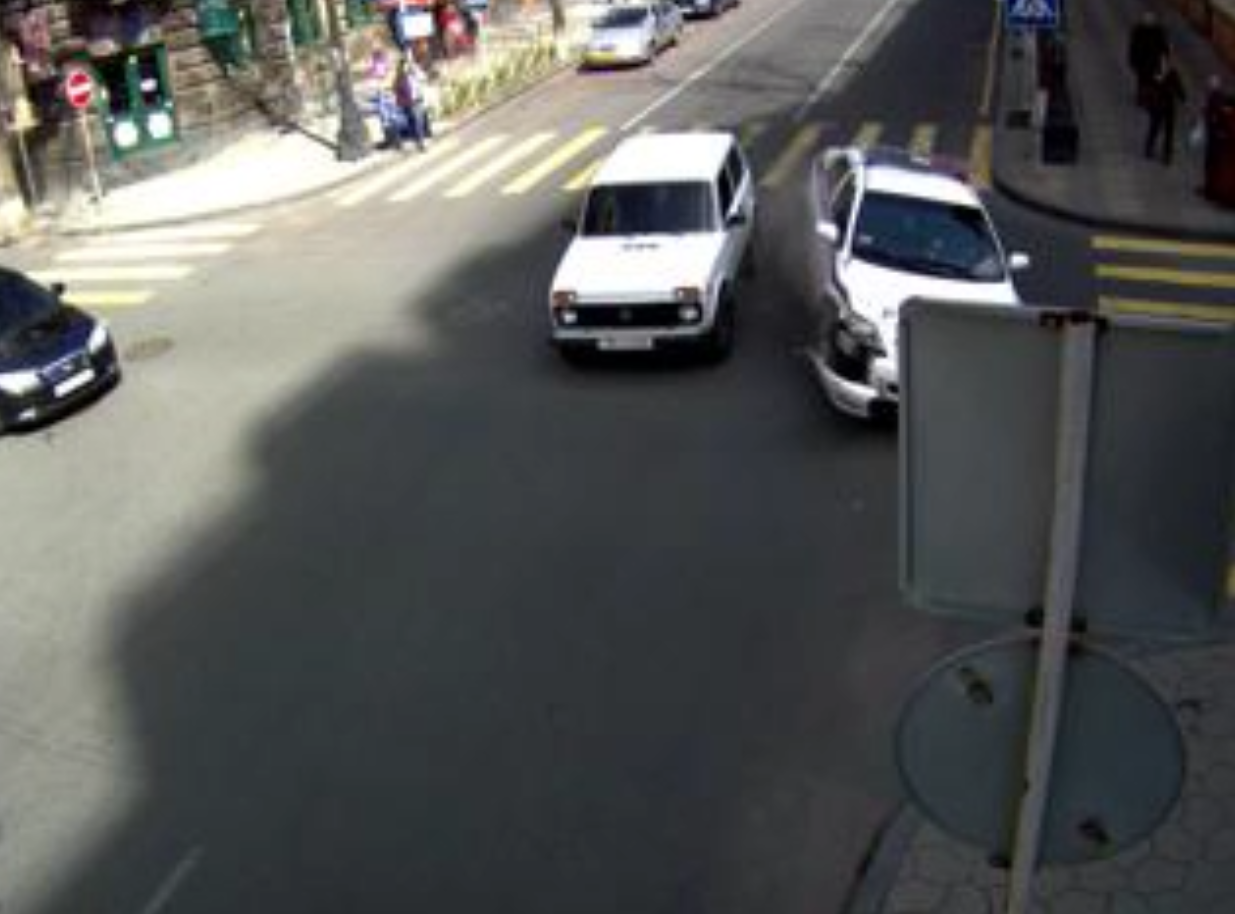
\includegraphics[width=\linewidth]{images/ucf/roadaccident-abnormal}
      \caption{Accidente}
    \end{subfigure}
  \end{figure}
\end{frame}

\begin{frame}{Modelo original}
  \begin{figure}
    \centering
    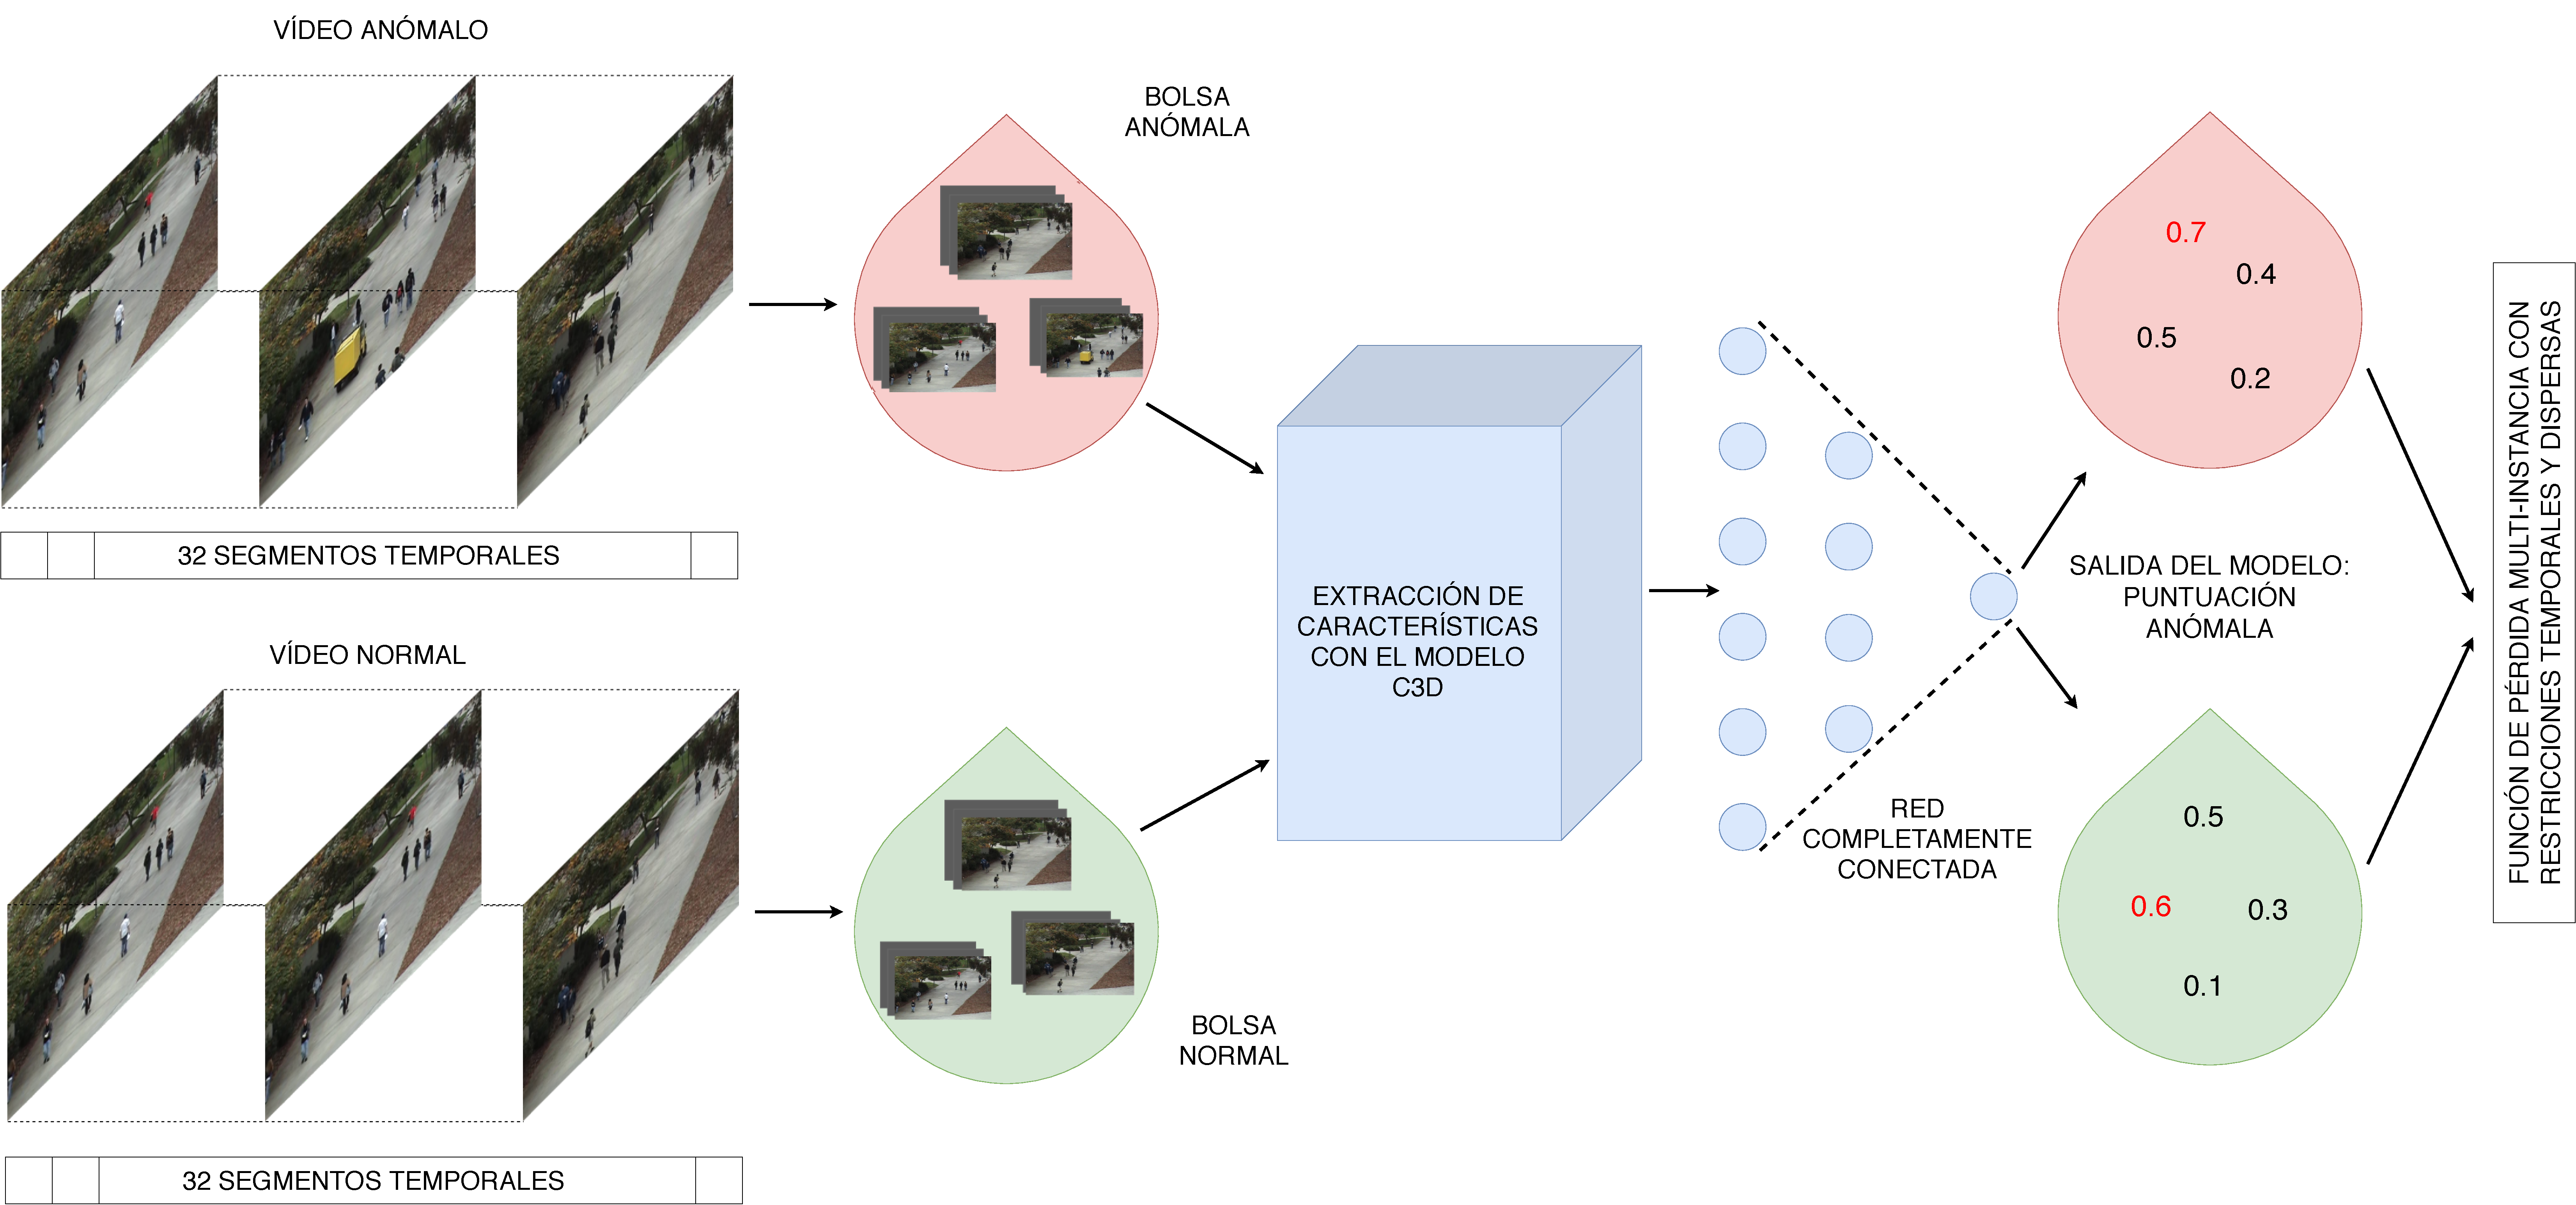
\includegraphics[width=.9\textwidth]{images/original-model.pdf}
    \caption{Modelo original}
  \end{figure}

  \blfootnote{Sultani, W., Chen, C., \& Shah, M. (2018). Real-world
    anomaly detection in surveillance videos. In Proceedings of the
    IEEE Conference on Computer Vision and Pattern Recognition
    (pp. 6479-6488).}
\end{frame}

\begin{frame}{Entrenamiento multiinstancia}
  \begin{block}{Entrenamiento del modelo}
    \begin{itemize}
    \item Una etiqueta por vídeo.
    \item Vídeos anómalos compuestos mayoritariamente por fotogramas normales.
    \item Predicción a nivel de fotograma.
    \end{itemize}
  \end{block}

  Solución: Función de pérdida multiinstancia
  \begin{align*}
    l(\mathcal{B}_a, \mathcal{B}_n)
    &= \max{(0, 1 - \max_{i \in \mathcal{B}_a}{f(\mathcal{V}^i_a)} +
      \max_{i \in \mathcal{B}_n}{f(\mathcal{V}^i_n)})}\\
    & + \lambda_1
      \sum_{i=0}^{n-1} (f(\mathcal{V}_a^i) - f(\mathcal{V}_a^{i+1})) +
      \lambda_2 \sum_{i=0}^{n} f(\mathcal{V}_a^i).
  \end{align*}

\end{frame}

\begin{frame}{Propuesta: Xception-LSTM}
  \begin{figure}
    \centering
    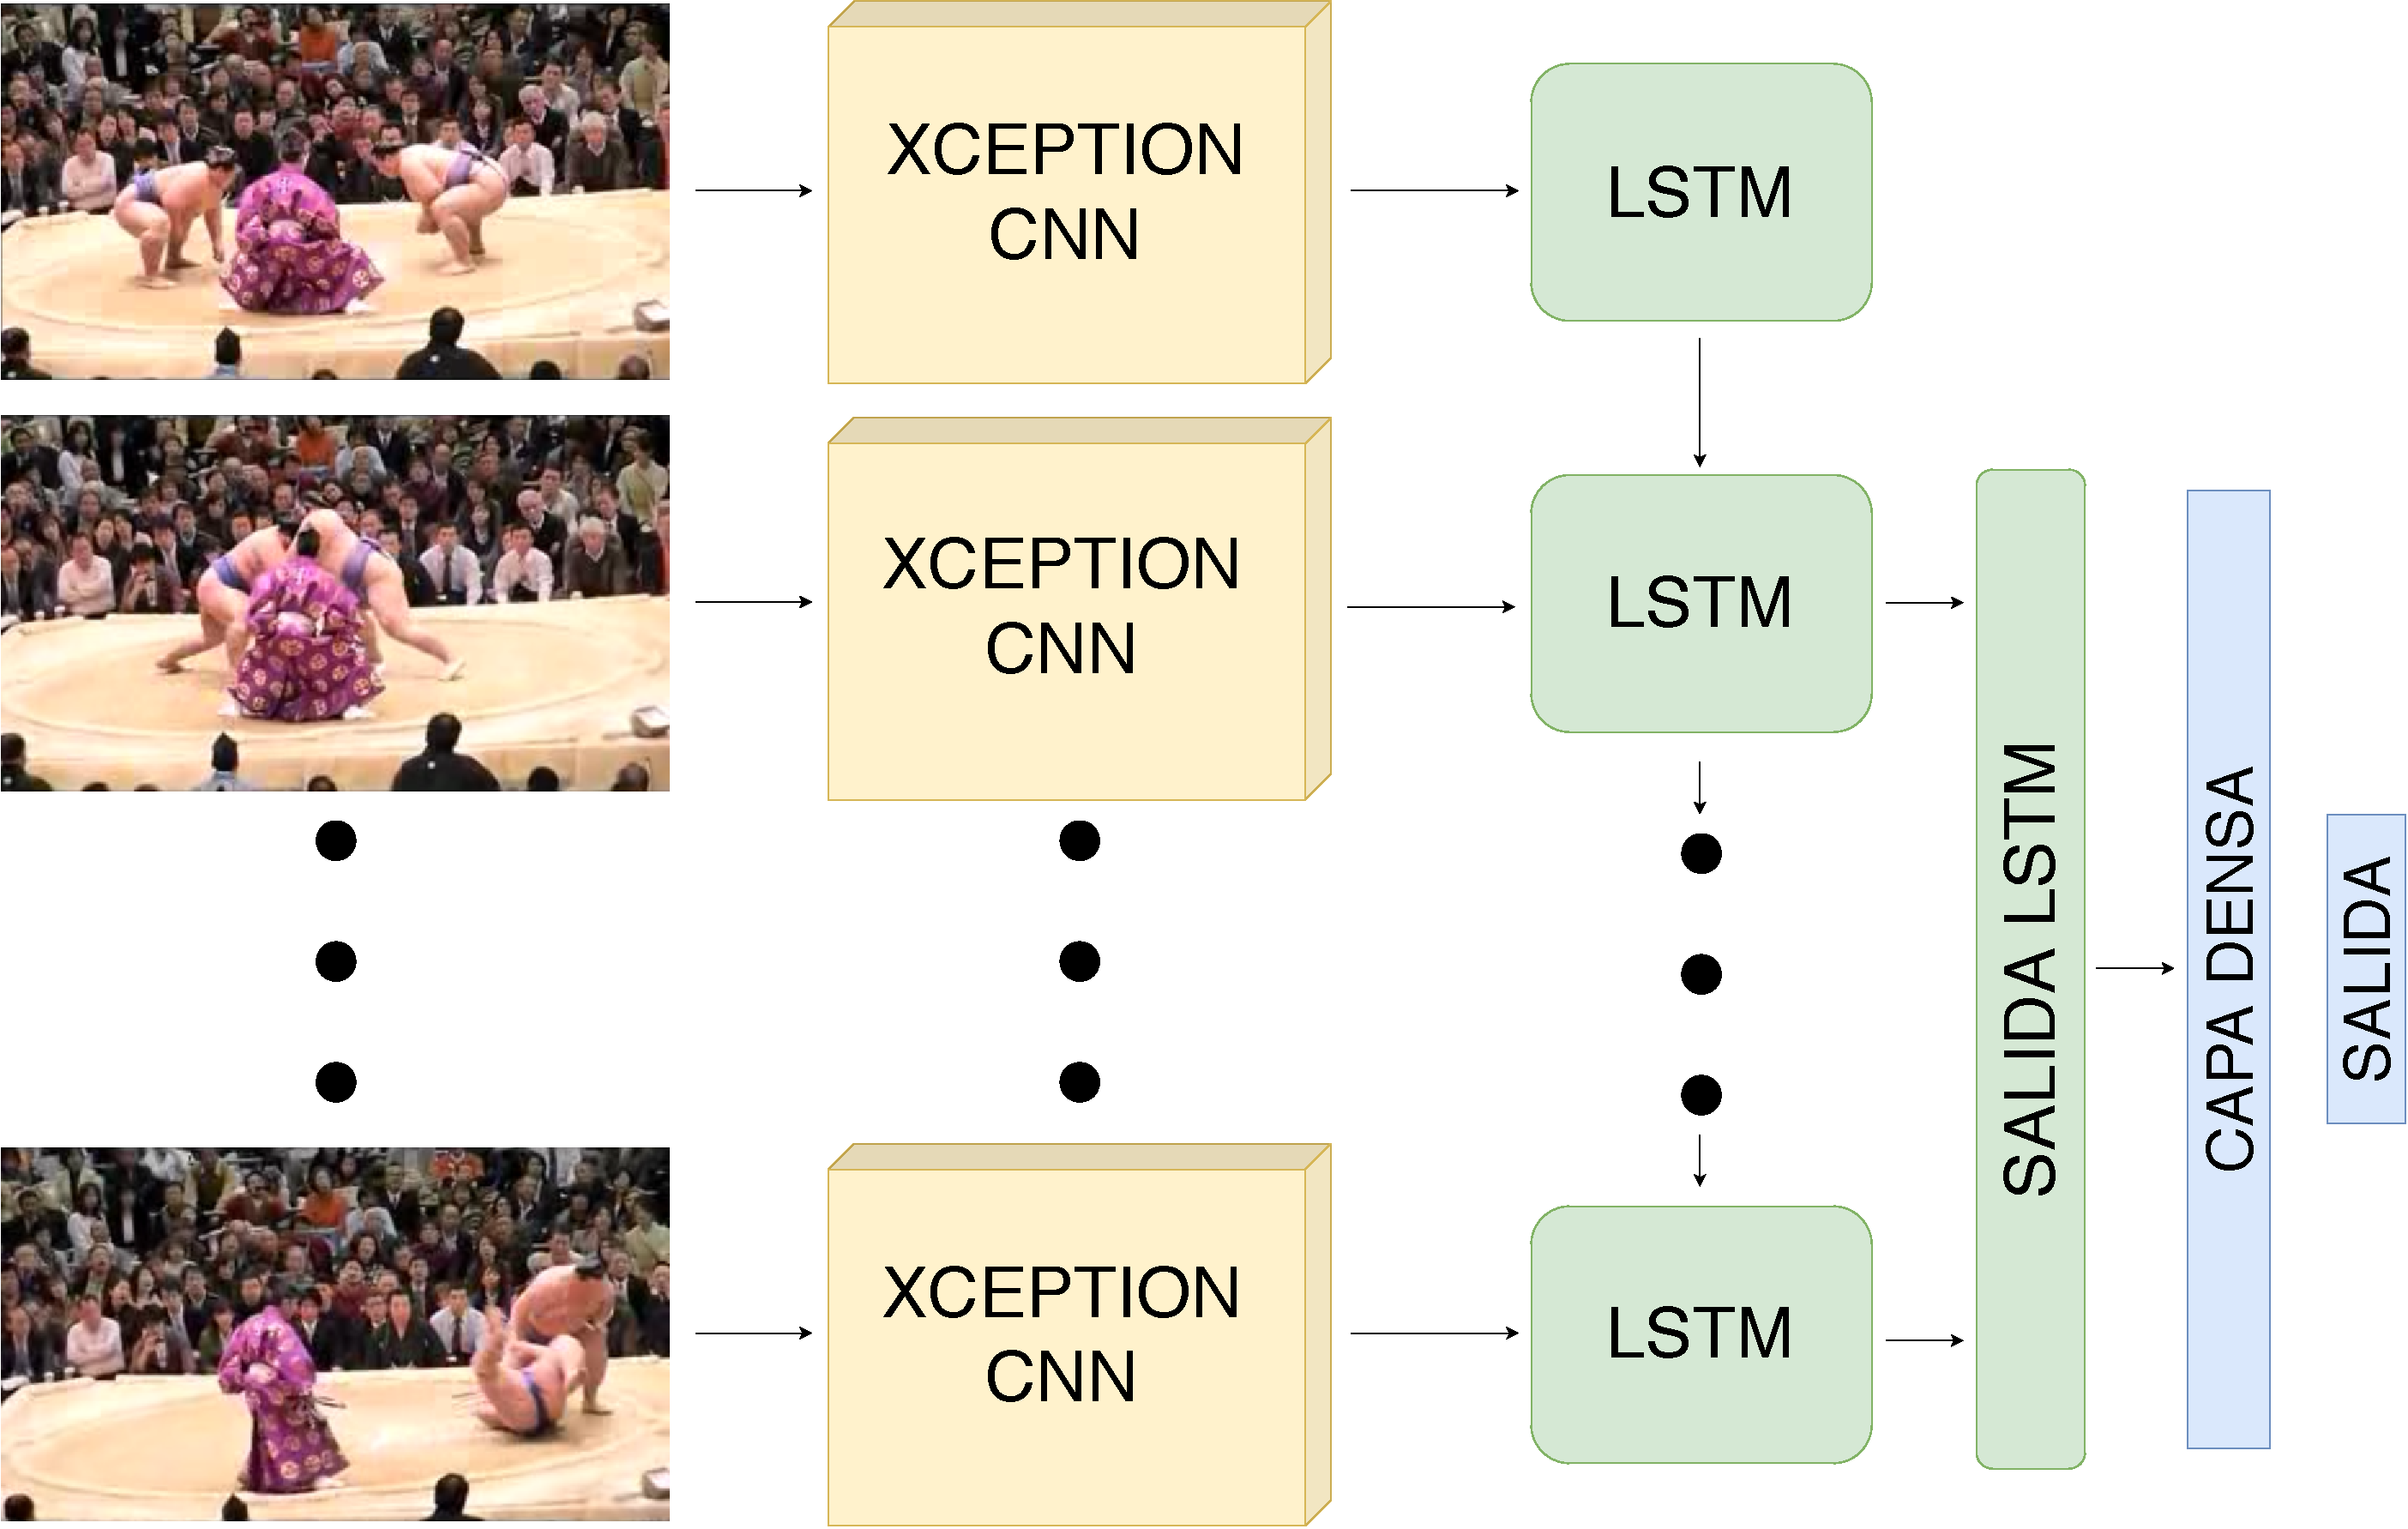
\includegraphics[width=.8\textwidth]{images/proposal.pdf}
    \caption{Arquitectura propuesta}
  \end{figure}
\end{frame}

\begin{frame}{Propuesta: Xception-LSTM}
  \begin{block}{Entrenamiento del modelo}
    \begin{itemize}
    \item Preentrenamiento del extractor: Clasificación sobre UCF-101
      (13000 vídeos, 101 clases).
    \item Congelación del extractor y extracción de características.
    \item Entrenamiento del clasificador.
    \end{itemize}
  \end{block}
\end{frame}

\section{Resultados}

\begin{frame}{Resultados a nivel de fotograma}
  \begin{table}[H]
    \centering
    \resizebox{\textwidth}{!}{
      \begin{tabular}{lccccc}
        \toprule
        Modelo & Exactitud & AUC & $F_1$ & EER & AP \\
        \midrule
        Original - preentrenado & 0.8428 & 0.7508 & 0.2838 & 0.3119 & \textbf{0.2057} \\
        Original - replicado & 0.7411 & 0.7369 & 0.2201 & 0.3253 & 0.2014 \\
        Xception-LSTM - 1024 & 0.8236 & 0.7504 & \textbf{0.2907} & 0.3221 & 0.1823 \\
        Xception-LSTM - 768 & \textbf{0.8455} & \textbf{0.7674} & 0.2681 & \textbf{0.2980} & 0.1770 \\
        Xception-LSTM - 512 & 0.8436 & 0.7177 & 0.2140 & 0.3388 & 0.1451 \\
        \bottomrule
      \end{tabular}
    }
    \caption{Tabla de resultados obtenidos por los modelos.}
    \label{tab:confusion-matrices}
  \end{table}
\end{frame}

\begin{frame}{Resultados a nivel de vídeo}
  \begin{table}[H]
    \centering
    \begin{tabular}{lcc}
      \toprule
      Modelo & \% Vídeos normales  & \% Vídeos anómalos \\
      \midrule
      Original & 13.33 & 64.89 \\
      Réplica & 11.11 & 74.05 \\
      Xception-LSTM - 1024 & 15.55 & \textbf{77.86} \\
      Xception-LSTM - 768 & 12.59 & 72.52 \\
      Xception-LSTM - 512 & \textbf{8.15} & 71.76 \\
      \bottomrule
    \end{tabular}
    \caption{Porcentaje de vídeos normales y anómalos en los que se ha
      generado una alarma.}
  \end{table}
\end{frame}

\begin{frame}{Ejemplo - Asalto}
  \begin{figure}
    \centering
    \animategraphics[loop,controls,width=.7\linewidth]{10}{images/gifs/assault-}{0}{132}
  \end{figure}
\end{frame}

\begin{frame}{Ejemplo - Robo}
  \begin{figure}
    \centering
    \animategraphics[loop,controls,width=.7\linewidth]{50}{images/gifs/stealing-}{000}{491}
  \end{figure}
\end{frame}

\section{Conclusiones y trabajo futuro}

\begin{frame}{Conclusiones y trabajo futuro}
  \begin{block}{Conclusiones}
    \begin{itemize}
    \item La detección de anomalías en multitudes es un problema
      complejo, debido a la diversidad de contextos a los que puede
      aplicarse.
    \item Los modelos espacio-temporales extraen características
      relevantes para la resolución de este problema, mejores que los
      modelos completamente convolucionales.
    \item Existe un margen de mejora amplio para este conjunto de datos.
    \end{itemize}
  \end{block}
  \begin{block}{Trabajo futuro}
    \begin{itemize}
    \item Despliegue del sistema en una aplicación real.
    \item Estudio de modelos ConvLSTM.
    \item Mejora de la política de entrenamiento del modelo.
    \end{itemize}
  \end{block}
\end{frame}

\begin{frame}[standout]
  \LARGE{Muchas gracias}\\
  \LARGE{¿Preguntas?}
\end{frame}

\end{document}
